\whiteBGstarBegin
\setcounter{section}{0}
\section{Trắc nghiệm}
\begin{enumerate}[label=\bfseries Câu \arabic*:]
	\item \mkstar{1}

\cauhoi
{Chuyển động thẳng đều là
	\begin{mcq}
		\item chuyển động thẳng, trong đó chất điểm có gia tốc không đổi.
		\item chuyển động có quỹ đạo là đường thẳng và có gia tốc như nhau trên mọi quãng đường.
		\item chuyển động có quỹ đạo là đường thẳng và có tốc độ trung bình như nhau trên mọi quãng đường.
		\item chuyển động thẳng, trong đó chất điểm có vận tốc tức thời thay đổi.
	\end{mcq}
}

\loigiai
{	\textbf{Đáp án: C.}
	
	Chuyển động thẳng đều là chuyển động có quỹ đạo là đường thẳng và có tốc độ trung bình như nhau trên mọi quãng đường.

}
\item \mkstar{1}

\cauhoi
{Phương trình chuyển động của chuyển động thẳng đều theo chiều dương là
	\begin{mcq}(2)
		\item $x=x_0+vt$ ($v<0$).
		\item $x=x_0-vt$ ($v<0$).
		\item $x=x_0+vt$ ($v>0$).
		\item $x=x_0-vt$ ($v>0$).
	\end{mcq}
}
\loigiai
{\textbf{Đáp án: A.}
	
	Phương trình chuyển động của chuyển động thẳng đều theo chiều dương là $x=x_0+vt$ ($v>0$).
}
\item \mkstar{1}

\cauhoi
{Phương trình chuyển động của chuyển động thẳng đều ngược chiều dương là
	\begin{mcq}(2)
		\item $x=x_0+vt$ ($v<0$).
		\item $x=x_0-vt$ ($v<0$).
		\item $x=x_0+vt$ ($v>0$).
		\item $x=x_0-vt$ ($v>0$).
	\end{mcq}
}
\loigiai
{\textbf{Đáp án: A.}
	
	Phương trình chuyển động của chuyển động thẳng đều ngược chiều dương là $x=x_0+vt$ ($v<0$).
}
\item \mkstar{2}

\cauhoi
{Phương trình chuyển động thẳng đều của một chất điểm có dạng $x=-4t+12$\\ ($x$: km, $t$: h). Quãng đường của chất điểm đi được sau $\SI{2}{\hour}$ là
	\begin{mcq}(4)
		\item $\SI{6}{\kilo\meter}$.
		\item $\SI{8}{\kilo\meter}$.
		\item $\SI{2}{\kilo\meter}$.
		\item $\SI{4}{\kilo\meter}$.
	\end{mcq}
}
\loigiai
{	\textbf{Đáp án: B.}	
	
	Quãng đường của chất điểm đi được sau $\SI{2}{\hour}$ là
	$$s=v_0t=\SI{4}{\kilo\meter/\hour}\cdot\SI{2}{\hour}=\SI{8}{\kilo\meter}.$$
}
\item \mkstar{2}

\cauhoi
{Một ôtô chuyển động trên một đoạn đường thẳng với tốc độ $\SI{60}{\kilo\meter/\hour}$. Bến xe nằm ở đầu đoạn đường nhưng xe xuất phát từ một điểm trên đoạn đường cách bến xe $\SI{4}{\kilo\meter}$. Chọn bến xe là vật mốc, chọn thời điểm xe xuất phát làm gốc thời gian và chọn chiều dương là chiều chuyển động. Phương trình chuyển động của ôtô trên đoạn đường này là
	\begin{mcq}(2)
		\item $x=60t$ (km, h).
		\item $x=4-60t$ (km, h).
		\item $x=4+60t$ (km, h).
		\item $x=-4-60t$ (km, h).
	\end{mcq}
	
}
\loigiai
{	\textbf{Đáp án: C.}
	
	Chọn bến xe là vật mốc, chọn thời điểm xe xuất phát làm gốc thời gian và chọn chiều dương là chiều chuyển động nên $x_0=\SI{4}{\kilo\meter}$, $v_0=\SI{60}{\kilo\meter/\hour}$.
	
	Phương trình chuyển động của ôtô trên đoạn đường này là: $x=4+60t$ (km, h).
}
\item \mkstar{2}

\cauhoi{
	Trên trục $\text O x$ có hai ô tô chuyển động với phương trình tọa độ lần lượt là $x_1 (t) = -20t+100\ (\text {m; s})$ và $x_2 (t) = 10t-50\ (\text {m; s})$. Khoảng cách giữa hai ô tô lúc $t=2\ \text s$ là
	\begin{mcq}(4)
		\item $\SI{90}{\meter}$.
		\item $\SI{0}{\meter}$.
		\item $\SI{60}{\meter}$.
		\item $\SI{30}{\meter}$.
	\end{mcq}
}
\loigiai
{	\textbf{Đáp án: A.}
	
	Tại thời điểm $t=2\ \text s$ thì các ô tô có tọa độ là $x_1 = \SI{60}{\meter}$, $x_2 = \SI{-30}{\meter}$.
	
	Khoảng cách giữa hai ô tô lúc $t=2\ \text s$ là $\SI{90}{\meter}$.
}
\item \mkstar{2}

\cauhoi{
	Lúc 7 giờ, một người ở A chuyển động thẳng đều với vận tốc $v=\SI{36}{\kilo \meter / \hour}$ đuổi theo người ở B đang chuyển động với vận tốc $v=\SI{5}{\meter / \second}$. Biết $\text{AB}=\SI{18}{\kilo \meter}$. Chọn gốc tọa độ ở A, chiều dương là chiều chuyển động. Phương trình chuyển động của người A và B lần lượt là
	\begin{mcq}(1)
		\item $x_\text A = 36t +18\ \text{(km, h)}$; $x_\text B = 18t\ \text{(km, h)}$.
		\item $x_\text A = 36t -18\ \text{(km, h)}$; $x_\text B = 18t + 18\ \text{(km, h)}$.
		\item $x_\text A = 36t\ \text{(km, h)}$; $x_\text B = 18t+18\ \text{(km, h)}$.
		\item $x_\text A = 36t\ \text{(km, h)}$; $x_\text B = 18t\ \text{(km, h)}$.
	\end{mcq}	
}
\loigiai
{	\textbf{Đáp án: C.}
	
		 Chọn gốc tọa độ ở A, chiều dương là chiều chuyển động.
	
	Phương trình chuyển động của người ở A: $x_\text A = 36t+0=36t\ \text{(km, h)}$.
	
	Phương trình chuyển động của người ở B (đổi $\SI{5}{\meter / \second} \rightarrow \SI{18}{\kilo \meter / \hour}$): $x_\text B = 18t+18\ \text{(km, h)} $.
}

\item \mkstar{3}

\cauhoi{Một xe chạy trong $\SI{5}{\hour}$, $\SI{2}{\hour}$ đầu xe chạy với tốc độ trung bình $\SI{60}{\km/\hour}$, $\SI{3}{\hour}$ sau xe chạy với tốc độ trung bình $\SI{40}{\km/\hour}$. Tốc độ trung bình của xe trong suốt thời gian chuyển động là
	\begin{mcq}(4)
		\item $\SI{48}{\kilo\meter/ \hour}$.
		\item $\SI{36}{\kilo\meter/ \hour}$.
		\item $\SI{54}{\kilo\meter/ \hour}$.
		\item $\SI{72}{\kilo\meter/ \hour}$.
	\end{mcq}
}
\loigiai
{	\textbf{Đáp án: A.}
	
	Quãng đường đi trong $\SI{2}{\hour}$ đầu là:
	$$s_1 = v_1t_1 = \SI{60}{\km/\hour}\cdot\SI{2}{\hour} = \SI{120}{km}.$$
	Quãng đường đi trong $\SI{3}{\hour}$ sau là:
	$$s_2 = v_2t_2 = \SI{40}{\km/\hour}\cdot\SI{3}{\hour} = \SI{120}{km}.$$
	Tốc độ trung bình của xe trong suốt thời gian chuyển động là:
	$$v_{\text{tb}}=\dfrac{s_1+s_2}{t_1+t_2}=\dfrac{\SI{120}{km}+\SI{120}{km}}{\SI{2}{\hour}+\SI{3}{\hour}}=\SI{48}{\km/\hour}.$$

}
\item \mkstar{4}

\cauhoi{ Vật chuyển động thẳng đều có đồ thị tọa độ - thời gian như hình vẽ. Phương trình chuyển động của vật có dạng nào sau đây?
	\begin{center}
		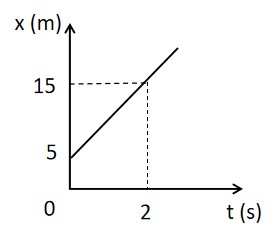
\includegraphics[scale=0.9]{../figs/VN10-2021-PH-TP003-1.jpg}
	\end{center}
	\begin{mcq}(4)
		\item $x=5+5t$.
		\item $x=4t$.
		\item $x=5-5t$.
		\item $x=5+4t$.
	\end{mcq}
}
\loigiai
{	\textbf{Đáp án: A.}
	
	Vận tốc của vật là:
	\begin{equation*}
		v=\dfrac{x-x_0}{t-t_0}=\dfrac{\SI{15}{\meter}-\SI{5}{\meter}}{\SI{2}{\second}}=\SI{5}{\meter/\second}.
	\end{equation*}
	
	Phương trình chuyển động của vật là:
	\begin{equation*}
		x=x_0+vt=5+5t\textrm{ (m, s)}.
	\end{equation*}
}

\item \mkstar{4}

\cauhoi{Một ô tô đi từ A đến B. Đầu chặng ô tô đi 1/4 tổng thời gian với $v_1=\SI{50}{\km/\hour}$. Giữa chặng ô tô đi 1/2 tổng thời gian với $v_2=\SI{40}{\km/\hour}$. Cuối chặng ô tô đi 1/4 tổng thời gian với $v_3=\SI{20}{\km/\hour}$. Tốc độ trung bình của ô tô là
	\begin{mcq}(4)
		\item $\SI{37,5}{\kilo\meter/\hour}$.
		\item $\SI{50,2}{\kilo\meter/\hour}$.
		\item $\SI{70}{\kilo\meter/\hour}$.
		\item $\SI{85}{\kilo\meter/\hour}$.
	\end{mcq}
}
\loigiai
{	\textbf{Đáp án: A.}
	
	Quãng đường ô tô đi đầu chặng là:
	$$s_1=v_1t_1=v_1\cdot\dfrac{t}{4}.$$
	Quãng đường ô tô đi giữa chặng là:
	$$s_2=v_2t_2=v_2\cdot\dfrac{t}{2}.$$
	Quãng đường ô tô đi cuối chặng là:
	$$s_3=v_3t_3=v_3\cdot\dfrac{t}{4}.$$
	Tốc độ trung bình của ô tô là:
	$$v_{\text{tb}}=\dfrac{s_1+s_2+s_3}{t}=\dfrac{v_1\cdot\dfrac{t}{4}+v_2\cdot\dfrac{t}{2}+v_3\cdot\dfrac{t}{4}}{t}=\dfrac{v_1}{4}+\dfrac{v_2}{2}+\dfrac{v_3}{4}=\SI{37,5}{\km/\hour}.$$
	
}

\end{enumerate}

\whiteBGstarEnd

\loigiai
{
	\begin{center}
		\textbf{BẢNG ĐÁP ÁN}
	\end{center}
	\begin{center}
		\begin{tabular}{|m{2.8em}|m{2.8em}|m{2.8em}|m{2.8em}|m{2.8em}|m{2.8em}|m{2.8em}|m{2.8em}|m{2.8em}|m{2.8em}|}
			\hline
			1.C  & 2.A  & 3.A  & 4.B  & 5.C  & 6.A  & 7.C  & 8.A  & 9.A  & 10.A  \\
			\hline
			
		\end{tabular}
	\end{center}
}
\section{Tự luận}
\begin{enumerate}[label=\bfseries Câu \arabic*:]
	\item \mkstar{1}
	
	\cauhoi{
		Chuyển đông thẳng đều là gì? Hãy cho biết biểu thức và ý nghĩa của tốc độ trung bình.
	}
	
	\loigiai{
		Chuyển động thẳng đều là chuyển động có quỹ đạo thẳng và có tốc độ trung bình như nhau trên mọi quãng đường.
		
		Tốc độ trung bình cho biết mức độ nhanh hay chậm của chuyển động. Công thức:
		$$v=\dfrac{s}{t}$$
	}
	
	\item \mkstar{2}
	
	\cauhoi{Nêu cách vẽ đồ thị tọa độ - thời gian của một chuyển động thẳng đều.}
	
	\loigiai{
		Để vẽ đồ thị $x-t$, ta cần xác định các cặp giá trị tương ứng $x$ và $t$ vào bảng.
		
		Vẽ hai trục tọa độ vuông góc: $\text O x$ là truc tung, $\text O t$ là trục hoành. Trên hệ $\text Oxt$ ta xác định các điểm $x$, $t$ trong bảng và nối các điểm đó lại với nhau.
	}
	\item \mkstar{3}
	
	\cauhoi
	{Đồ thị tọa độ - thời gian cho bên dưới.
		\begin{center}
			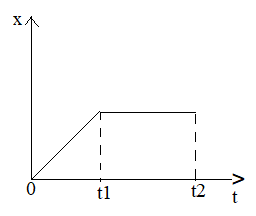
\includegraphics[scale=0.9]{../figs/VN10-2021-PH-TP0003-2.png}
		\end{center}
	
	Hãy mô tả chuyển động của chất điểm trong khoảng thời gian từ ban đầu đến $t_1$ và từ $t_1$ đến $t_2$.
	}
	
	\loigiai
	{Từ lúc $t=0$ đến $t_1$: vật chuyển động thẳng đều theo chiều dương.
		
		Từ lúc $t_1$ đến $t_2$: vật đứng yên.
	}
	\item \mkstar{4}
	
	\cauhoi
	{Một người đi xe đạp trên đoạn đường AB. Nửa đoạn đường đầu người ấy đi với vận tốc $v_1=\SI{20}{km/h}$. Trong quãng thời gian còn lại thì một nửa quãng thời gian đầu người đó đi với vận tốc $v_2=\SI{10}{km/h}$, một nửa quãng thời gian cuối người đó đi với vận tốc $v_3=\SI{5}{km/h}$. Tính vận tốc trung bình trên cả đoạn đường AB. 
	}
	
	\loigiai
	{
	Vận tốc trung bình trên cả đoạn đường:
	$$v=\dfrac{2}{\dfrac{1}{v_1}+\dfrac{1}{v_2}}$$
	
	Vận tốc trung bình trên nửa đoạn đường thứ hai:
	$$v_2=\dfrac{v_2'+v_2''}{2} = \SI{7.5}{km/h}$$
	
	Vậy vận tốc trung bình trên cả đoạn đường:
	$$v=\SI{10.9}{km/h}$$
	}
	\item \mkstar{4}
	
	\cauhoi
	{Một chiếc ô tô chạy từ điểm A đến điểm B. Nửa đoạn đường đầu ô tô đi với vận tốc $v_1=\SI{40}{km/h}$. Trong quãng thời gian còn lại thì một nửa quãng thời gian đầu ô tô đi với vận tốc $v_2=\SI{50}{km/h}$, một nửa quãng thời gian cuối ô tô đi với vận tốc $v_3=\SI{60}{km/h}$. Tính vận tốc trung bình của ô tô trên cả đoạn đường AB.
	}
	
	\loigiai
	{	Vận tốc trung bình trên cả đoạn đường:
		$$v=\dfrac{2}{\dfrac{1}{v_1}+\dfrac{1}{v_2}}$$
		
		Vận tốc trung bình trên nửa đoạn đường thứ hai:
		$$v_2=\dfrac{v_2'+v_2''}{2} = \SI{55}{km/h}$$
		
		Vậy vận tốc trung bình trên cả đoạn đường:
		$$v=\SI{57.4}{km/h}$$
	}
\end{enumerate}